\chapter{实验过程}

在本次毕业设计 “面向智慧交通场景的多目标跟踪算法和评测” 中,多目标跟踪技术是实现关键功能的核心技术之一。本次研究通过在 CARLA 仿真平台的 Town10 场景中开展实验,对现有的多目标跟踪模型进行优化,并对其性能进行评估。借助跟踪到的小车轨迹数据,提升复现的性能指标。具体步骤如下。

\section{基础控制}
\subsection{轨迹平滑控制}

如果小车预设路径里,相邻两个航点间距过大,小车开起来会显得很别扭,很不自然,精确控制难度也会增加。轨迹平滑算法可以在原始路径点之间添加一些额外的点,让小车轨迹变得顺滑,这样一来,小车的运动就会流畅很多如图\ref{fig:p9}。


\begin{figure}[htbp] % 可以是h(here),t(top),b(bottom),p(page of floats)
	\centering
	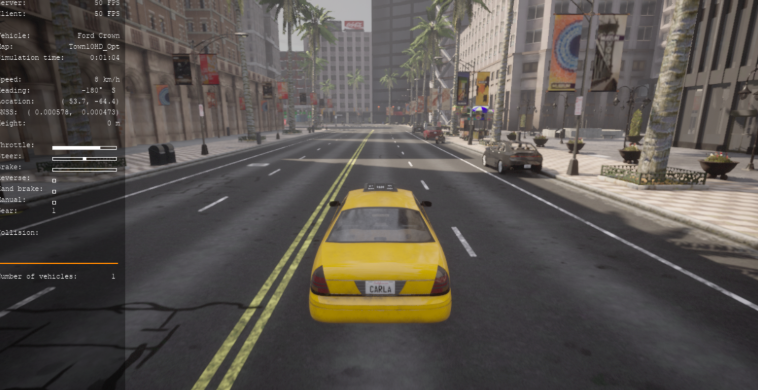
\includegraphics[width=1\textwidth]{p9} % 假设图片文件名为car.pdf或car.png等,位于当前工作目录
	\caption{轨迹平滑控制} % 图片标题
	\label{fig:p9} % 用于引用的标签
\end{figure}






\subsection{实现步骤}

确定最小距离阈值:根据小车的运动学特性和仿真环境的要求,设定一个最小距离阈值,本项目最初在Carla环境里选择的0.5米。

需要计算插值点时,先逐个查看原始路径点。如果发现相邻两点间距大于设定的最小距离阈值,就计算它们之间的插值点。这里可以用线性插值,根据两点坐标和距离,按固定步长插入中间点。

生成平滑路径:将原始路径点和插值点按照顺序组合成新的平滑路径,作为小车的实际行驶轨迹,发送给小车的控制系统。

\subsection{PID 控制}
采用PID控制算法,由比例控制(P)、积分控制(I)、微分控制(D)三个部分组成,对车辆进行控制,使得车辆按预先生成的轨迹行驶到达目的地。先通过对实现小车的基本控制来为后续的开发与测试做出铺垫。本次设计的PID控制的具体计算公示与逻辑如图\ref{fig:p17}所示。


\begin{figure}[htbp] % 可以是h(here),t(top),b(bottom),p(page of floats)
	\centering
	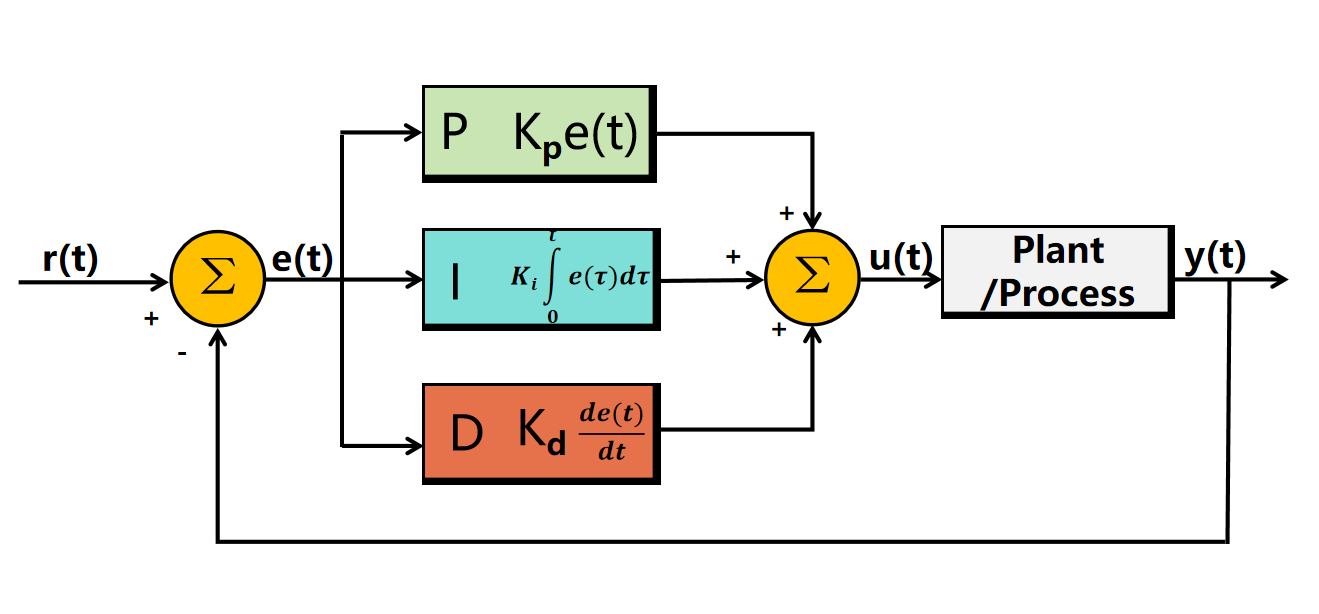
\includegraphics[width=1\textwidth]{p17} % 假设图片文件名为car.pdf或car.png等,位于当前工作目录
	\caption{PID 控制} % 图片标题
	\label{fig:p17} % 用于引用的标签
\end{figure}






\section{基于雷达和相机获取小车坐标数据}
在实现了对小车的基础控制之后,接下来就需要通过结合相机与雷达传感器,利用CARLA仿真平台进行多目标跟踪,获取车辆在多个路口的精确轨迹,并通过再识别技术整合整体轨迹,实现对车辆的精准控制,从而构建完整的车辆数字孪生系统。以下便是步骤。

\subsection{激光雷达检测}

本次设计用 CARLA 的激光雷达和摄像头做数据融合来跟踪车辆,获取车辆相对于自家车的轨迹,为此得用 CARLA 的雷达数据集训练 pointPillars 网络。本次设计在收集轨迹跟踪数据时,在 Town10 场景里运行 collect lidar dataset.py 脚本收集点云训练集,训练集包括点云数据和 3D 标签框,都放在 . /multi obj track 文件夹下,方便后续开发管理。脚本先分别创建存雷达数据和标签数据的文件夹,过滤掉自行车等非目标车辆的蓝图,把车辆分为 “car”和 “truck”两类。接着获取雷达检测范围内的车辆信息,将其转换到雷达坐标系下,并保存为 MATLAB 格式的标签文件,将雷达点云数据转换为 NumPy 数组,并保存为 MATLAB 可以读取的格式,然后配置并启动激光雷达传感器,绑定回调函数以保存数据,最后销毁销毁传感器和车辆。

\subsubsection{点云数据预处理}
在MATLAB中,执行`convertTrainPointCloudToPcd.m`脚本,先获取并确保相关文件夹路径正确,再获取数据文件夹下的 .mat 文件列表,接着逐个加载这些文件,提取点云数据构建 pointCloud 对象,然后按激光雷达参数重组点云数据,最后将重组后的点云以 ASCII 格式的 PCD 文件保存,将点云训练集转换为PCD格式文件;同时运行`convertTrainLabelToTableMat.m`脚本,先初始化空表格并获取、确认相关文件夹路径正确,再获取数据文件夹下的 .mat 文件列表,接着逐个加载文件,提取汽车和卡车的标签数据并转换为表格行添加到主表格中,最后将主表格保存为 CarlaSetLidarGroundTruth.mat 文件,将所有帧的训练标签整合为一个MAT文件。最后将会得到如图\ref{fig:p10}展示的数据文件。




\begin{figure}[htbp] % 可以是h(here),t(top),b(bottom),p(page of floats)
	\centering
	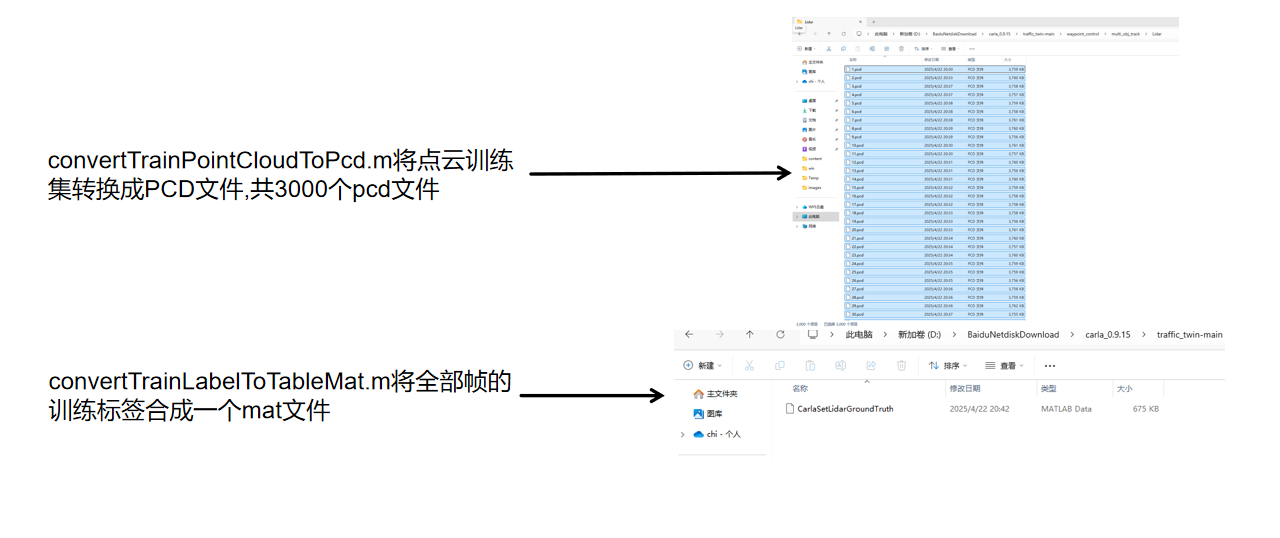
\includegraphics[width=1\textwidth]{p10} % 假设图片文件名为car.pdf或car.png等,位于当前工作目录
	\caption{点云数据预处理} % 图片标题
	\label{fig:p10} % 用于引用的标签
\end{figure}




\subsubsection{训练}
在matlab中运行pointPillarsTrain.m脚本,开始训练如图\ref{fig:p30}!先设置数据路径,加载雷达点云数据和边界框标签,并展示全视图点云;接着定义裁剪参数,裁剪点云并处理标签;然后拆分数据集为训练集和测试集,保存训练数据为 PCD 文件,创建文件数据存储和框标签数据存储并合并用于训练;之后通过过采样和变换对点云数据增强,增加数据集多样性;再计算锚框,创建 PointPillars 模型;设置训练参数,训练模型并保存检查点;从测试集取点云进行目标检测,可视化检测结果;最后保存训练好的检测模型。将训练好的模型如图\ref{fig:p11}保存在当前目录(./multi obj track)下。



\begin{figure}[htbp] % 可以是h(here),t(top),b(bottom),p(page of floats)
	\centering
	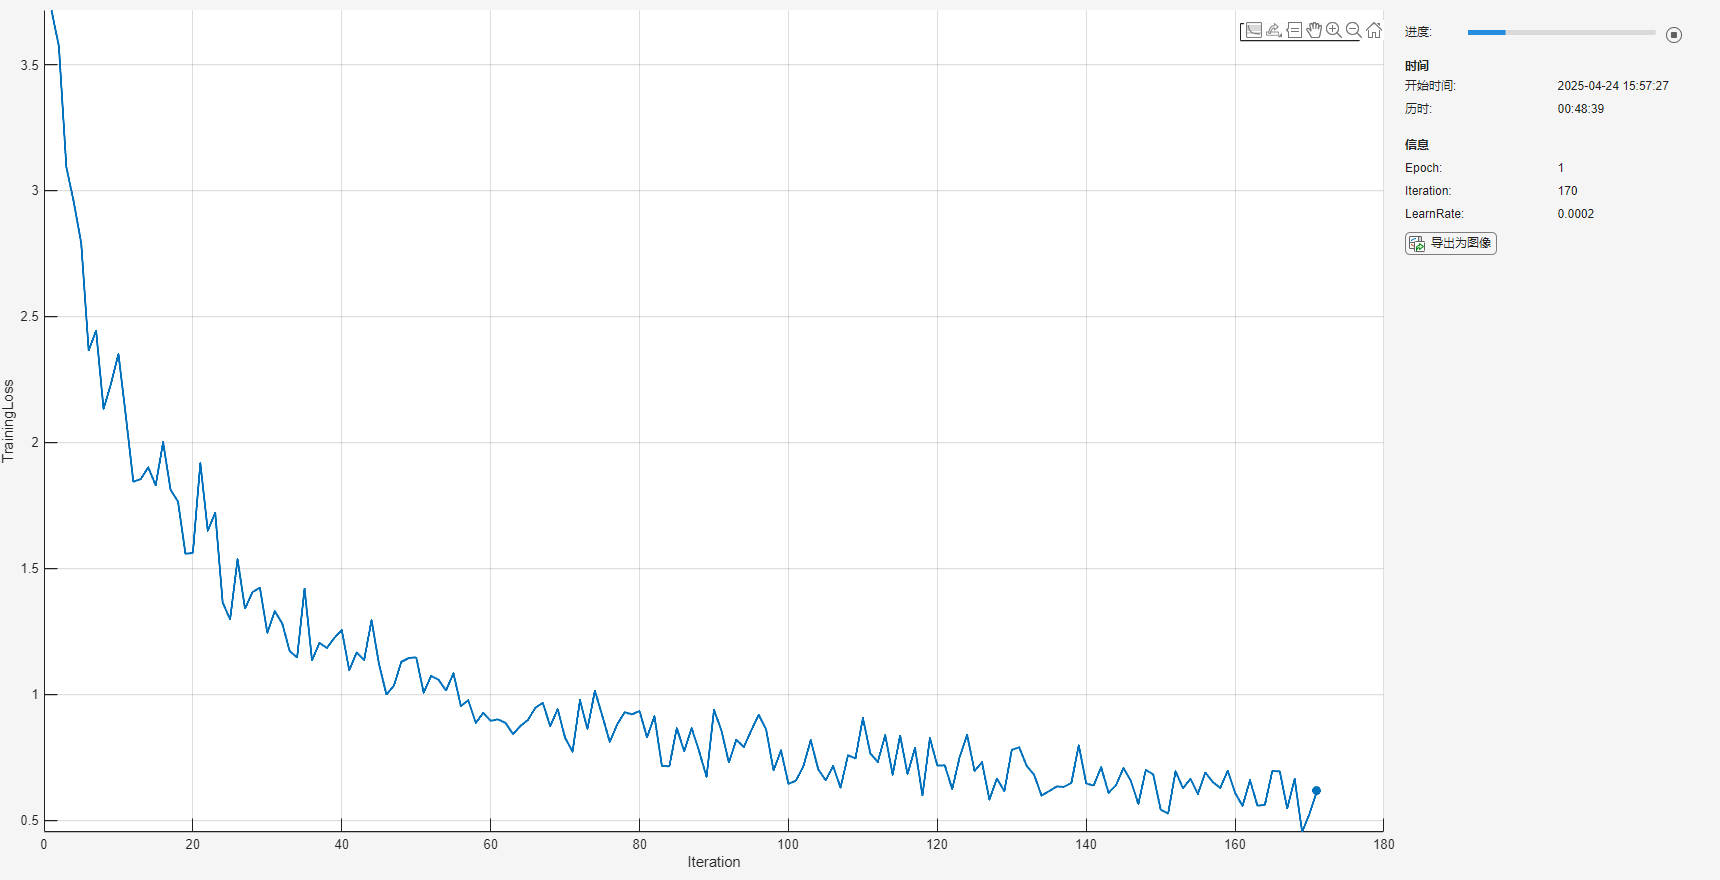
\includegraphics[width=1\textwidth]{p30} % 假设图片文件名为car.pdf或car.png等,位于当前工作目录
	\caption{模型训练中} % 图片标题
	\label{fig:p30} % 用于引用的标签
\end{figure}








\begin{figure}[htbp] % 可以是h(here),t(top),b(bottom),p(page of floats)
	\centering
	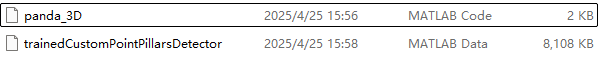
\includegraphics[width=1\textwidth]{p11} % 假设图片文件名为car.pdf或car.png等,位于当前工作目录
	\caption{训练好的模型} % 图片标题
	\label{fig:p11} % 用于引用的标签
\end{figure}






\subsection{激光雷达和摄像头数据的对象级融合}
\subsubsection{收集轨迹跟踪的数据}
在Town10场景,运行collect intersection camera lidar.py收集多目标跟踪的测试数据,其中每个路口中心包括1个激光雷达,雷达周围覆盖6个RGB相机,收集每一帧的6个视角的场景图片和点云数据,放在./multi obj track下。在collect intersection camera lidar.py脚本中,设置DATA MUN = 500,意思是收集500帧的6个视角的场景图片和点云数据如图\ref{fig:p12},用于以后的操作。



\begin{figure}[htbp] % 可以是h(here),t(top),b(bottom),p(page of floats)
	\centering
	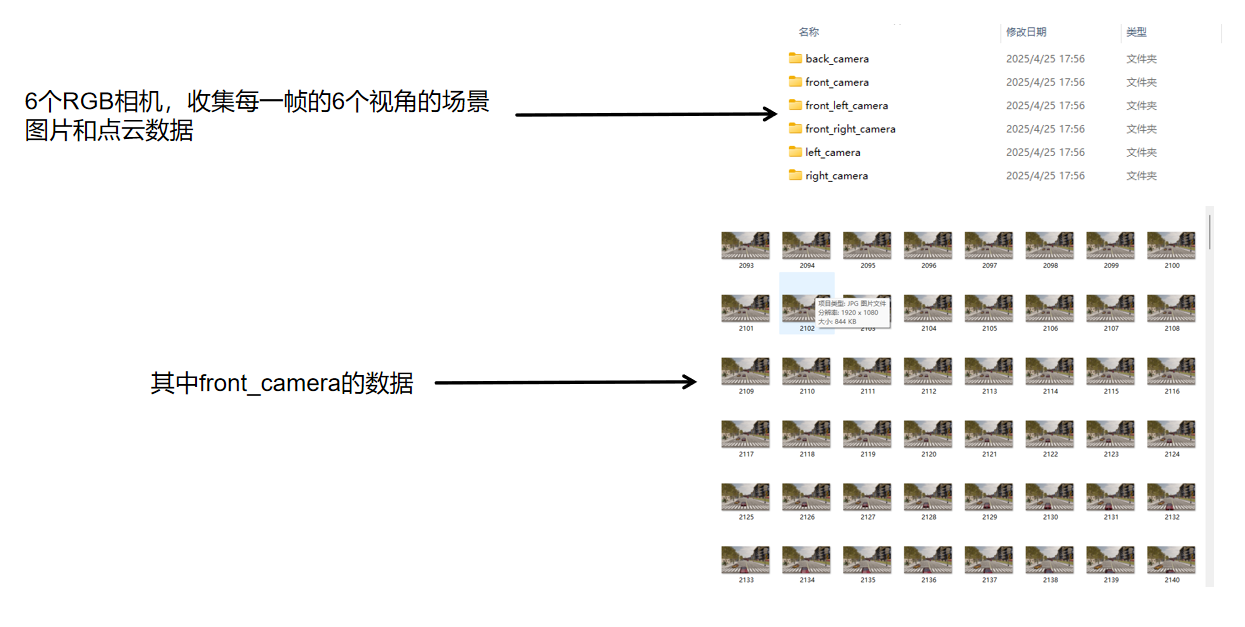
\includegraphics[width=1\textwidth]{p12} % 假设图片文件名为car.pdf或car.png等,位于当前工作目录
	\caption{雷达相机数据} % 图片标题
	\label{fig:p12} % 用于引用的标签
\end{figure}



\subsubsection{数据预处理}


detect3DBoundingBox.m 这个程序是用来在点云数据里找车并给它们打上3D标签的。首先,它会从指定的地方加载提前训练好的PointPillars检测模型。接着,它会获取某个文件夹里所有的.mat文件。对每个文件,它会先检查有没有有效的点云数据。要是有,就提取出来并整理成点云对象。之后,用检测模型来找目标,得到边界框、置信度和标签,并把这些结果显示出来,最后再存回到原来的文件里。

detect2DBoundingBox.m 这个程序是用来在图片里找车并给它们打上2D标签的,这里直接用了预训练好的YOLOv4模型。先初始化YOLOv4检测器,然后获取指定文件夹里的所有.mat文件。对每个文件检查有没有datalog变量,如果有,就一个一个看相机数据并读取图片。用YOLOv4检测器找目标,不过会把“traffic light”标签的检测结果过滤掉。最后把有用的检测结果存回原始文件。



\subsubsection{数据融合,获取轨迹}
multiObjectTracking.m可视化跟踪的车辆。先进行路径配置与文件加载,初始化显示与轨迹对象;然后在数据帧处理循环中,依次进行数据加载与时间戳检查、提取检测数据、检测结果融合、目标跟踪、结果可视化、轨迹更新与保存;最后将完整轨迹数据保存至指定文件夹以便后续评估与分析,输出trackedData.mat。
\subsubsection{坐标转换}
获取的轨迹是相对于自车的坐标,然而本次设计假设自车是静止在路口中间(实际不存在),雷达和相机都附着在自车上,也就是说与自车存在一个相对位置,示例中雷达与车辆的相对位置是[0,0,0],但本项目中雷达是高出一定的距离。convertTrackToCarlaCoordinate.m将坐标转换成CARLA场景中的轨迹,使用的是相对于自车的,因此(x,y)是正确的。


经过以上(1)~(4)的步骤便可以得到500帧如图\ref{fig:p13}所示(在collect intersection camera lidar.py中设置的参数DATA MUN = 500)的收集轨迹跟踪视频。



\begin{figure}[htbp] % 可以是h(here),t(top),b(bottom),p(page of floats)
	\centering
	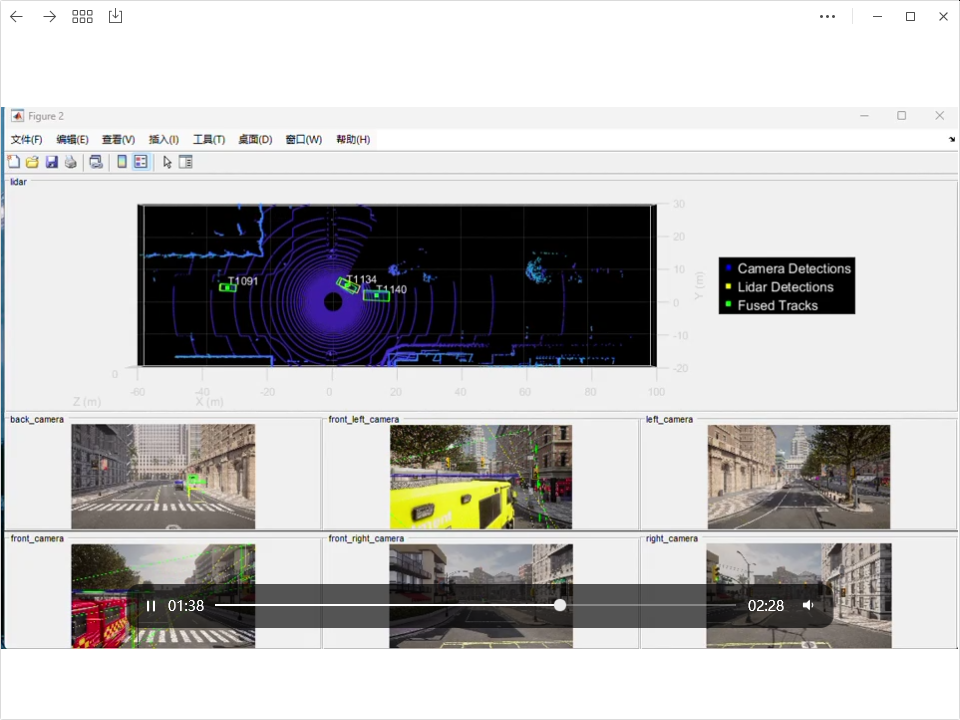
\includegraphics[width=1\textwidth]{p13} % 假设图片文件名为car.pdf或car.png等,位于当前工作目录
	\caption{收集轨迹跟踪视频其中一帧} % 图片标题
	\label{fig:p13} % 用于引用的标签
\end{figure}







\subsection{Re-ID网络再识别}
\subsubsection{收集车辆再识别数据集}
通过使用collect reid dataset.py在相同的位置生成车辆,在车辆起点和终点位置分别放一个RGB相机和一个语义分割相机,获取每一帧的车辆头部和尾部方向的图片以及2D标签。
\subsubsection{数据裁剪}
运行cropReIDDataSet.m将前后视角的车辆图片根据2D标签进行裁剪,并且将同一类型车辆两个视角的图片整合到一起,最后reshape为224 \times 224的大小如图\ref{fig:p14}。



\begin{figure}[htbp] % 可以是h(here),t(top),b(bottom),p(page of floats)
	\centering
	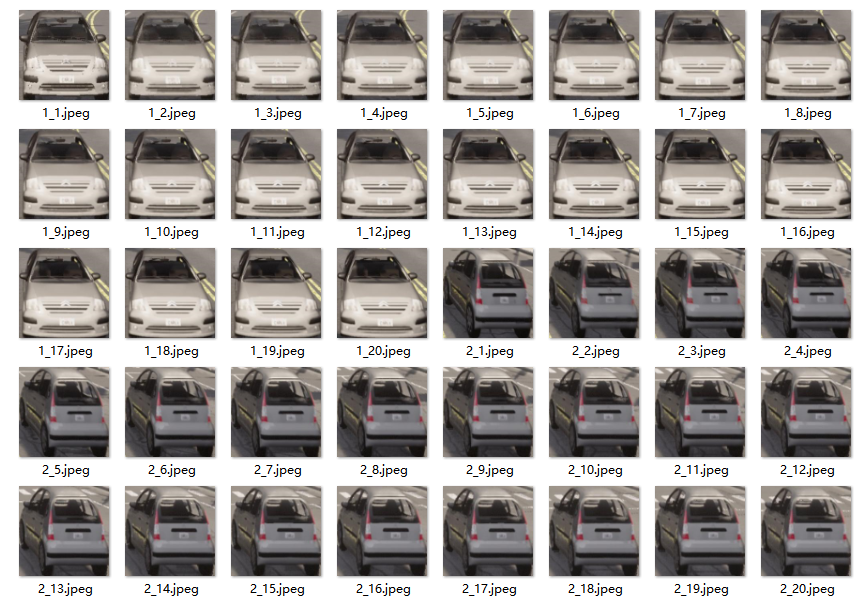
\includegraphics[width=1\textwidth]{p14} % 假设图片文件名为car.pdf或car.png等,位于当前工作目录
	\caption{裁剪后的数据} % 图片标题
	\label{fig:p14} % 用于引用的标签
\end{figure}




\subsubsection{训练}
reIDNetworkTrain.m改用 imagePretrainedNetwork 函数并指定 resnet50 模型进行训练,该神经网络已基于大量图像学习了丰富的特征表示。
\subsubsection{测试}
将路口1位置跟踪到的车辆车辆图片和路口2位置该视角相机的图片放在一起进行再识别reIdentification.m, 也就是说第一张图是要重新识别的对象,在下个路口进行识别,进而整合二者的轨迹,最终便可以得到如图\ref{fig:p15}再识别后的数据。







\begin{figure}[htbp] % 可以是h(here),t(top),b(bottom),p(page of floats)
	\centering
	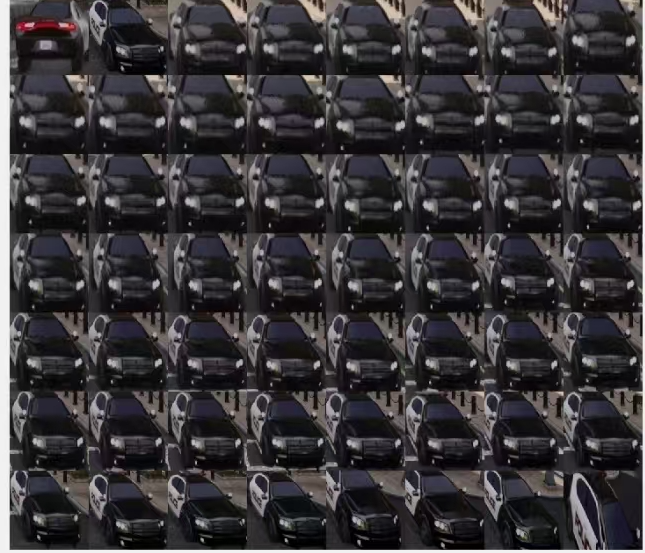
\includegraphics[width=1\textwidth]{p15} % 假设图片文件名为car.pdf或car.png等,位于当前工作目录
	\caption{再识别后数据} % 图片标题
	\label{fig:p15} % 用于引用的标签
\end{figure}









\subsection{路口间车辆轨迹匹配}
\subsubsection{生成可作匹配的轨迹}
多目标跟踪multiObjectTracking.m可视化跟踪的车辆,输出trackedData.mat的同时,也保存了每条轨迹所对应车辆的图片,该图片是通过结合所融合的3D框和Yolo识别的2D框判断为同一辆车后,选择该2D框进行裁剪,重塑生成可作特征提取的224×224大小的图片。

loadAllTraj.m 用于生成指定路口轨迹,包括该轨迹对应车辆的外观特征。
\subsubsection{车辆轨迹匹配}
目前是仅是通过计算两个路口间全部轨迹所对应车辆的余弦相似度来匹配,若路口1有M辆车,路口2有N辆车,则生成M×N的矩阵,其中大于一定的阈值,则判定两辆车为同一辆车。
\subsubsection{运行}
执行DEMO.m,先加载配置文件并设置路径,接着加载各路口的轨迹文件到 cell 数组,然后通过匹配算法将不同路口的轨迹按阈值链接成完整路径,最后保存匹配后的轨迹实现将两个路口的轨迹进行关联!
\subsection{重复上述步骤}
因为本课题中要求是关于多路口的目标跟踪检测,上述操作只包含了road intersection 1路口的内容。与此同时Town10地图中有6个路口,所以还需返回到激光雷达和摄像头数据的对象级融合中第一步“收集轨迹跟踪的数据”中重新运行collect intersection camera lidar.py,在这个脚本中将road intersection 1改成road intersection 2(后续可以改写成3或4或5)以此来收集其他路口的数据。最终收集完整的数据如图\ref{fig:p18}所示。




\begin{figure}[htbp] % 可以是h(here),t(top),b(bottom),p(page of floats)
	\centering
	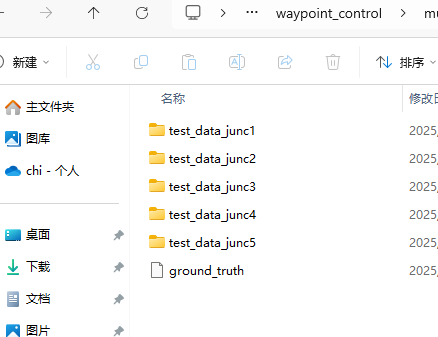
\includegraphics[width=1\textwidth]{p18} % 假设图片文件名为car.pdf或car.png等,位于当前工作目录
	\caption{五个路口数据} % 图片标题
	\label{fig:p18} % 用于引用的标签
\end{figure}






\section{小车轨迹复现}

通过在上述描述的步骤中,已经通过收集road intersection 1、road intersection 2、road intersection 3、road intersection 4和road intersection 5这五个路口的小车坐标数据。


\subsection{对轨迹数据的优化}
由于项目中的雷达摄像头是介于路口与路口之间的,其中可能没有小车路口转弯或者直走的轨迹,也可能观察不到小车路口转弯或者直走的轨迹。所以项目中的evaluator.py程序用来使用动态时间规整(DTW)计算两个路口摄像头对小车轨迹的重合度。
\subsubsection{计算两条轨迹的重合度}
首先提取轨迹的 x, y 坐标,确保两条轨迹长度一致(取较短的长度),使用 DTW 计算轨迹之间的距离,计算最大可能距离((假设两条轨迹完全不重合)。计算他们的重合度,并且限制重合度在 [0, 1] 之间。
使用动态时间规整(DTW)计算两条轨迹的重合度。

param truth trajectory: 真实轨迹,格式为 [[x1, y1, t1], [x2, y2, t2], ...]。

param track trajectory: 控制轨迹,格式为 [[x1, y1, z1], [x2, y2, z2], ...]。

param threshold: 判断重合点的位置误差阈值(默认 0.5 米)。

return: 轨迹重合度(0 到 1 之间的值,1 表示完全重合)。

\subsubsection{计算轨迹的多个指标}
其次计算轨迹的多个指标,本项目做法是先遍历 truth 和 track 的键和值,初始化当前车辆的指标,再计算当前车辆的误差计算欧氏距离(仅考虑 x 和 y),计算当前车辆的轨迹重合度(使用 DTW),计算当前车辆的终点误差,接着累加当前车辆的指标并且计算平均指标。

平均轨迹重合度(Mean Trajectory Overlap Ratio, TOR)

平均位置误差(Mean Position Error, MPE)

平均最大位置误差(Mean Maximum Position Error, MeanMaxPE)

平均终点误差(Mean Final Position Error, MFPE)

param truth: 车辆的轨迹字典,键为车辆编号,值为 [[x1, y1, t1], [x2, y2, t2], ...]。

param track: 控制车辆所走的轨迹字典,键为车辆编号,值为 [[x1, y1, z1], [x2, y2,z2], ...]。

param threshold: 判断重合点的位置误差阈值(默认 0.5 米)。

return:平均轨迹重合度、平均位置误差、平均最大位置误差和平均终点误差的元组(mean tor,mean error, mean max error, mean fpe)。


\subsubsection{计算所有车辆的误差}
最后遍历每辆车的横向误差、纵向误差和延迟列表(如果车辆没有数据,跳过),确保横向误差、纵向误差和延迟的帧数一致,加当前车辆的横向误差、纵向误差和延迟,算平均横向误差、平均纵向误差和平均延迟(如果没有数据,返回 (0.0, 0.0, 0.0))。

计算所有车辆的平均横向误差(Mean Lateral Error, MLE)、平均纵向误差(Mean Longitudinal Error, MLOE)和平均延迟(Mean Delay, MD)。

param lateral errors: 横向误差列表,每个子列表表示一辆车的每一帧的横向误差。

param longitudinal errors: 纵向误差列表,每个子列表表示一辆车的每一帧的纵向误差。

param delays: 延迟列表,每个子列表表示一辆车的每一帧的延迟。

return:平均横向误差、平均纵l向误差和平均延迟的元组(mean lateral error,mean longitudinal error, mean delay)。


\subsection{坐标数据再处理}
\subsubsection{多路口车辆轨迹数据}

将五个路口全部轨迹全部放在DEMO.m脚本下运行,DEMO.m脚本首先加载轨迹数据,对每个路口的数据集路径,使用 loadAllTraj 函数加载该路口的所有轨迹数据,通过遍历所有 .mat如图\ref{fig:p19}(test data junc1 traj、test data junc2 traj、test data junc3 traj、test data junc4 traj、test data junc5 traj) 文件,加载每个文件中的轨迹数据,并将其存储在 juncTrajCell 中。接着对轨迹匹配及保存,matchThreshold 定义了车辆轨迹匹配的阈值,用于判断不同路口的轨迹是否属于同一辆车,在完成该步骤之后调用 linkIdentities 函数,将所有路口的轨迹数据进行匹配和链接,生成全局唯一的车辆轨迹。最后将匹配后的轨迹数据保存到名为 traj.mat 的文件中。

总的来说,这段代码用于处理多路口的车辆轨迹数据,通过匹配和链接生成全局唯一的轨迹,便于后续对车辆轨迹的复现。



\begin{figure}[htbp] % 可以是h(here),t(top),b(bottom),p(page of floats)
	\centering
	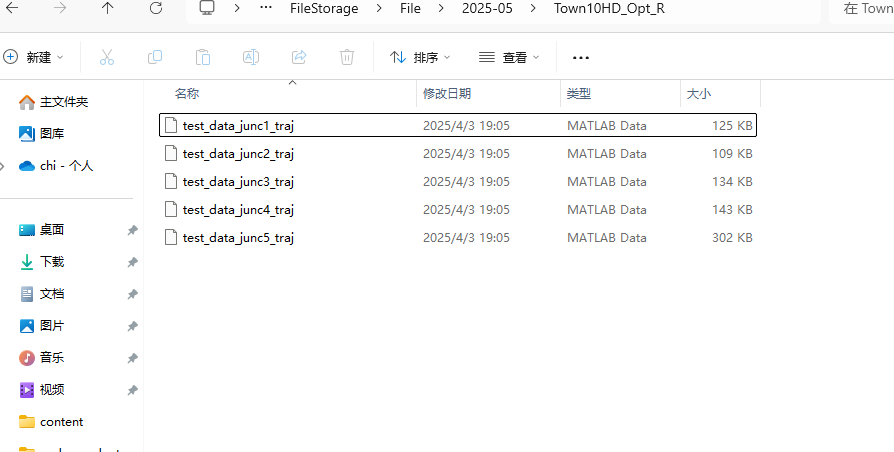
\includegraphics[width=1\textwidth]{p19} % 假设图片文件名为car.pdf或car.png等,位于当前工作目录
	\caption{五个路口数据} % 图片标题
	\label{fig:p19} % 用于引用的标签
\end{figure}






\subsubsection{转化轨迹数据格式}
对于以上步骤得到的五个路口车辆轨迹坐标数据,还无法满足本项目对车辆轨迹的复现,在Drive.py脚本中,在对车辆轨迹复现时,读取的车辆轨迹数据是名为 Waypoints.txt 文件夹中的数据。还需要将上文得到的五个路口车辆轨迹坐标数据转化为int(float或double)类型的坐标数据存入Waypoints.txt中。

项目先对小车轨迹处理,从traj.mat文件加载车辆轨迹数据,每个轨迹含三维坐标点和时间戳。检查轨迹起点,若离道路过远就过滤。同一车辆在多路口出现的轨迹,用Carla路径规划生成中间路径,插值确保时间戳连续。用fastdtw算法算跟踪轨迹与真实轨迹最优匹配,评估指标有平均位置误差、最大位置误差、最终位置误差和轨迹重合度。最后,将处理后的车辆轨迹按时间戳排序,存入Waypoints.txt文件,如图\ref{fig:p20}所示。


\begin{figure}[htbp] % 可以是h(here),t(top),b(bottom),p(page of floats)
	\centering
	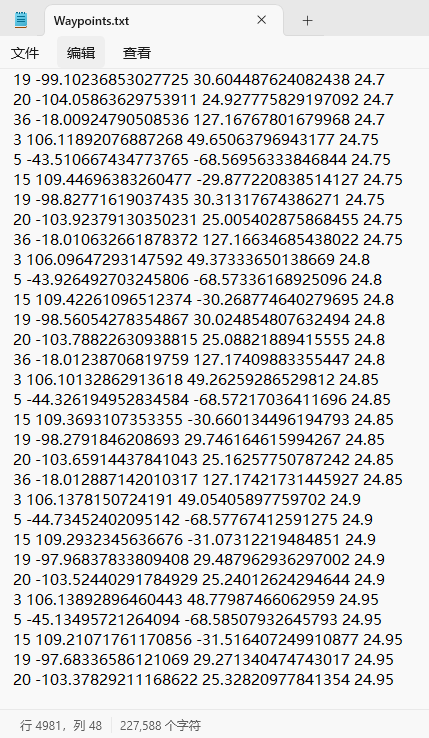
\includegraphics[width=0.5\textwidth]{p20} % 假设图片文件名为car.pdf或car.png等,位于当前工作目录
	\caption{小车坐标轨迹数据} % 图片标题
	\label{fig:p20} % 用于引用的标签
\end{figure}









\subsection{开始复现}

通过以上的准备工作,项目已经具有能力去预估介于路口与路口之间其中可能没有小车路口转弯或者直走的轨迹,也可能观察不到小车路口转弯或者直走的轨迹。所以在Drived.py脚本中,调用Waypoints.txt中小车坐标数据,在已经通过evaluator.py程序进行优化与预测的情况下。运行Drived.py脚本,完成对小车轨迹的复现如图\ref{fig:p21}所示,该图片只展示了本次设计复现视频过程中的其中一帧,让小车的basedline达到课题规定的5\%以上的要求。



\begin{figure}[htbp] % 可以是h(here),t(top),b(bottom),p(page of floats)
	\centering
	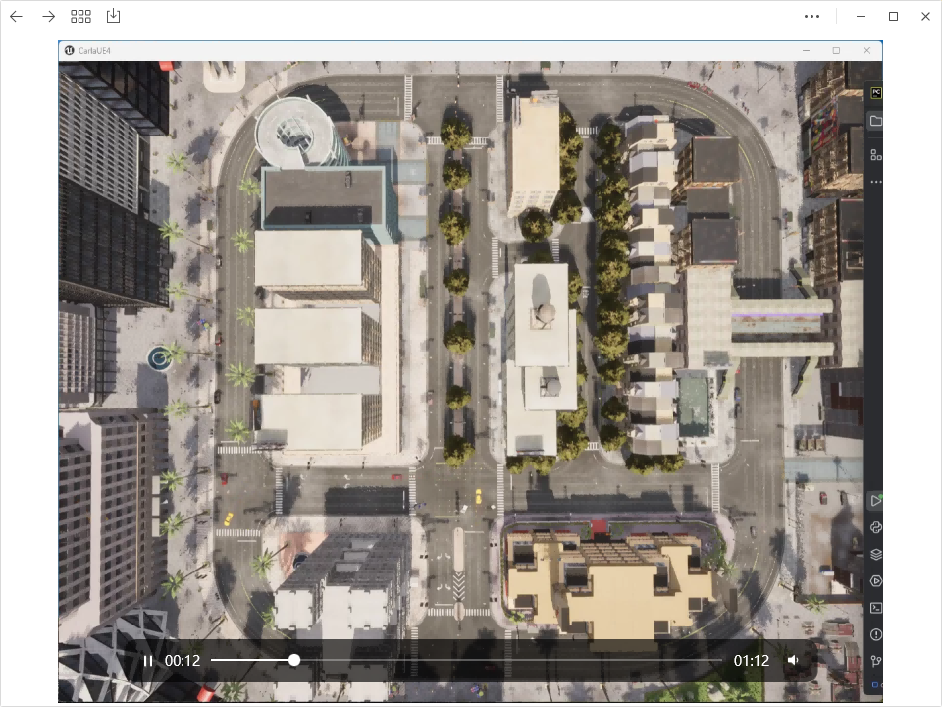
\includegraphics[width=1\textwidth]{p21} % 假设图片文件名为car.pdf或car.png等,位于当前工作目录
	\caption{小车轨迹的复现} % 图片标题
	\label{fig:p21} % 用于引用的标签
\end{figure}






\section{结果分析}

本次毕业设计研究的是面向智慧交通场景的多目标跟踪算法和评测,主要对检测跟踪模型做了优化,在很多性能指标上都实现了明显提升。实验结果显示,优化后的模型在 MOTA、MOTP 和 IDS 这些关键指标上,都比 Baseline 高出了 5\%。此外,还通过可视化方法直观地呈现了模型优化后的效果。
接下来,本次设计便展示性能指标与优化目标,还有模型优化与结果分析。








\subsection{结果性能分析}
\subsubsection{性能指标}
TT(Trajectory Tracking):轨迹跟踪,是指控制车辆沿着给定轨迹行驶,轨迹定义在时间域上,需要同时控制车辆的横向和纵向运动,以贴合给定轨迹并匹配其时间。

DT(Detection and Tracking):检测与跟踪,这类方法依赖于从传感器数据(如摄像头、激光雷达等)中检测车辆,然后对检测到的车辆进行跟踪,以生成轨迹。

GT(Generation and Tracking):生成与跟踪,这可能涉及使用预测模型或轨迹生成算法来生成车辆的预期轨迹,然后将这些生成的轨迹与实际跟踪数据相结合,以提高轨迹预测的准确性和完整性。

TOR(Trajectory Overlap Rate):轨迹重合度,表示跟踪轨迹与真实轨迹的重合程度,通常用来衡量轨迹跟踪的准确性。

MPE(Mean Position Error):平均位置误差,指跟踪轨迹与真实轨迹之间位置误差的平均值,用于评估轨迹跟踪的精度。

MaxPE(Maximum Position Error):最大位置误差,指跟踪轨迹与真实轨迹之间位置误差的最大值,用于评估轨迹跟踪中最坏情况下的误差。

FPE(Final Position Error):最终位置误差,指跟踪轨迹与真实轨迹在轨迹终点的位置误差,用于评估轨迹跟踪的最终精度。

MLE(Mean Longitudinal Error):平均纵向误差,指沿轨迹方向的纵向误差的平均值,用于评估车辆在纵向上的跟踪精度。

MLOE(Mean Lateral Offset Error):平均横向偏移误差,指垂直于轨迹方向的横向偏移误差的平均值,用于评估车辆在横向上的跟踪精度。

MD(Mean Deviation):平均偏差,指跟踪轨迹与真实轨迹之间的平均偏差,综合反映了轨迹跟踪的整体误差水平。

MOTA(Multi-Object Tracking Accuracy):多目标跟踪精度,综合考虑了跟踪的准确性和完整性。

MOTP(Multi-Object Tracking Precision):多目标跟踪精度,衡量跟踪轨迹与真实轨迹的匹配程度。

Int.(Intersection):意为“交叉路口”或“交汇点”。

IDS:综合考虑了跟踪的准确性和稳定性的指标。

FP(False Positives):误检数量。

FN(False Negatives):漏检数量。

MT(Mostly Tracked):大部分时间被跟踪的目标数量。

ML(Mostly Lost):大部分时间丢失的目标数量。

Fragmentation:轨迹碎片化程度。

Precision:精确率。

Recall:召回率。
\subsubsection{优化目标}
根据课题要求,优化后的模型至少在3个性能指标上超过Baseline的5\%。本次设计通过改进检测算法、优化数据融合策略和引入更先进的跟踪算法,实现了对现有模型的优化。







\subsection{模型优化}

检测算法改进:使用PointPillars深度学习模型进行激光雷达3D目标检测,并结合预训练的YOLOv4模型进行2D目标检测,提高了检测的准确性和速度。

数据融合策略优化:通过激光雷达和摄像头数据的对象级融合,利用卡尔曼滤波器对目标轨迹进行平滑处理,减少了轨迹碎片化现象。

跟踪算法改进:引入了基于ReID(Re-Identification)的再识别技术,通过计算车辆外观特征的余弦相似度,实现了在多个路口间的车辆轨迹匹配,提高了跟踪的稳定性和准确性。

\subsubsection{模型优化一:跟踪}

过插值算法使轨迹点更加平滑和连续,以填补轨迹中的空白或减少冗余点,从而提高轨迹跟踪的准确性和流畅性。

利用Carla的全局路径规划器计算车辆在不同位置之间的最短路径,为轨迹跟踪提供更合理的路径规划。

使用动态时间规整(DTW)算法计算跟踪轨迹与真实轨迹之间的相似度,从而评估轨迹跟踪的准确性和鲁棒性。

计算多种轨迹跟踪指标,如平均轨迹重合度(TOR)、平均位置误差(MPE)、平均最大位置误差(MeanMaxPE)和平均终点误差(MFPE),以便全面评估轨迹跟踪的效果。

通过对优化前后的模型进行评测,得到了以下如表~\ref{tab:trajectory_com}和如表~\ref{tab:tracking_comparison}性能指标的统计结果:

\begin{table}[h]
	\centering
	\caption{Trajectory Overlap Rate and Vehicle Control Indicators}
	\label{tab:trajectory_com}
	\resizebox{\textwidth}{!}{%
		\begin{tabular}{|l|c|c|c|c|c|c|c|c|c|c|c|c|c|}
			\hline
			\textbf{Scene} & \textbf{Int.} & \textbf{Rcll} & \textbf{Prcn} & \textbf{FTR} & \textbf{FP} & \textbf{FN} & \textbf{IDS} & \textbf{MT} & \textbf{ML} & \textbf{RMOTA} & \textbf{RMOTP} \\ \hline
			\multicolumn{12}{|c|}{优化后 Town10} \\ \hline
			Town10  & 1 & 30.1025 & 59.9258 & 0.5106 & 216 & 750 & 18 & 0.0000 & 37.5000 & 8.2945 & 79.9222 \\ \hline
			Town10  & 2 & 64.8065 & 61.5385 & 1.1027 & 450 & 391 & 21 & 55.5556 & 33.3333 & 22.4122 & 86.7746 \\ \hline
			Town10  & 3 & 63.2135 & 45.4407 & 1.1887 & 359 & 174 & 15 & 0.0000 & 25.0000 & -15.8562 & 86.9053 \\ \hline
			Town10  & 4 & 65.8206 & 96.7662 & 0.0369 & 13 & 202 & 20 & 40.0000 & 20.0000 & 60.2369 & 89.0919 \\ \hline
			Town10  & 5 & 41.4035 & 90.0763 & 0.0580 & 13 & 167 & 10 & 50.0000 & 0.0000 & 33.3333 & 88.2471 \\ \hline
			\multicolumn{12}{|c|}{优化前 Town10} \\ \hline
			Town10  & 1 & 30.6653 & 59.7166 & 0.7960 & 398 & 1334 & 28 & 8.3333 & 50.0000 & 8.5239 & 84.6488 \\ \hline
			Town10  & 2 & 56.4410 & 70.6095 & 1.1380 & 569 & 1055 & 29 & 13.3333 & 2666467 & 31.7506 & 81.0192 \\ \hline
			Town10  & 3 & 51.9805 & 75.6714 & 0.6160 & 308 & 885 & 17 & 14.2857 & 35.7143 & 34.3464 & 84.2826 \\ \hline
			Town10  & 4 & 52.1930 & 86.1427 & 0.2680 & 134 & 763 & 50 & 27.2727 & 36.3636 & 40.6642 & 88.6035 \\ \hline
			Town10  & 5 & 45.4243 & 62.2719 & 1.6540 & 827 & 1640 & 35 & 12.5000 & 37.5000 & 16.7388 & 86.0825 \\ \hline
		\end{tabular}
	}
\end{table}


\begin{table}[htbp]
	\centering
	\caption{Multi-objective Tracking Evaluation Comparison}
	\label{tab:tracking_comparison}
	\begin{tabular}{@{}llcccccc@{}}
		\toprule
		\textbf{Scene} & \textbf{Metric} & \textbf{Optimized Town10} & \textbf{Before Optimization Town10} \\
		\midrule
		\multirow{8}{*}{Town10} 
		& Rcll & 64.8065 (Int. 2) & 86.1427 (Int. 4) \\
		& Pren & 61.5385 (Int. 2) & 86.1427 (Int. 4) \\
		& FTR & Better in Int. 1 and 2 & Generally lower, 52.4243 (Int. 5) \\
		& FP & Lower in Int. 3 and 5 & Higher in Int. 1 and 2 \\
		& FN & Higher in Int. 3 and 4 & Higher in Int. 1 and 3 \\
		& IDS & Fewer & 35 (Int. 5) \\
		& MT & Better in Int. 2 and 3 & 40.0000 (Int. 4) \\
		& RMOTA/RMOTP & 79.9222 (RMOTP, Int. 2) & 84.2826 (RMOTP, Int. 4) \\
		\bottomrule
	\end{tabular}
\end{table}



综合对比:
如果重视 跟踪准确率(Rcll) 和 精确率(Pren),优化前Town10 在高密度和复杂地形场景(如第三个和第四个路口)中表现更好。
如果重视 特征轨迹召回率(FTR) 和 假阳性率(FP),优化后Town10 在平坦道路和稀疏建筑场景(如第一个和第二个路口)中表现更优。
身份切换(IDS) 和 大部分轨迹(MT) 指标显示,优化后Town10 在目标身份稳定性和持续跟踪方面具有一定优势。
在 RMOTA 和 RMOTP 综合指标方面,优化后Town10 和 优化前Town10 在不同路口各有亮点,但 优化后Town10 整体略占优势。














\subsubsection{模型优化二:复现}

通过收集车辆的外观特征(如不同角度的图像)和语义分割信息,为轨迹复现提供了更丰富的外观特征,有助于在不同场景下准确识别和复现车辆的轨迹。

通过加载和处理多个路口的轨迹数据,并使用匹配算法将不同路口的轨迹链接起来,生成全局唯一的车辆轨迹,从而优化了轨迹复现的完整性和连续性。

提供了评估轨迹复现质量的指标和方法,如通过计算轨迹重合度、位置误差等指标,可以量化评估轨迹复现的准确性和可靠性,从而指导对轨迹复现算法的优化。


通过对优化前后的模型进行评测,得到了以下表~\ref{tab:trajectory_comparisons}和表~\ref{tab:trajectory_comparison}性能指标的统计结果:


\begin{table}[h]
	\centering
	\caption{Trajectory Overlap Rate and Vehicle Control Indicators}
	\label{tab:trajectory_comparisons}
	\resizebox{\textwidth}{!}{%
		\begin{tabular}{|c|c|c|c|c|c|}
			\hline
			\textbf{Scene} & \textbf{Type} & \textbf{TOR(\%)} & \textbf{MPE(m)} & \textbf{MaxPE(m)} & \textbf{FPE(m)} \\ \hline
			优化前 Town10 & TT-DT & 50.2143 & 79.5798 & 33.1382 & 19.8970 \\ \hline
			& TT-GT & 18.4326 & 59.3773 & 79.6541 & 64.0980 \\ \hline
			& Control & MLE: 2.1889, MLOE: 0.5345, MD: 1.2015 \\ \hline
			优化后 Town10 & TT-DT & 10.8957 & 82.4108 & 105.8893 & 105.0854 \\ \hline
			& TT-GT & 34.4533 & 52.5575 & 36.0566 & 31.4600 \\ \hline
			& Control & MLE: 1.9835, MLOE: 0.2614, MD: 1.3780 \\ \hline
		\end{tabular}
	}
\end{table}


\begin{table}[htbp]
	\centering
	\caption{Trajectory Tracking Performance Comparison}
	\label{tab:trajectory_comparison}
	\begin{tabular}{@{}lcccccc@{}}
		\toprule
		\textbf{Scene} & \textbf{Type} & \textbf{TOR(\%)} & \textbf{MPE(m)} & \textbf{MaxPE(m)} & \textbf{FPE(m)} \\
		\midrule
		\multicolumn{2}{l}{\textbf{Optimized Town10}} \\
		\quad TT-DT & & 10.8957 & 82.4108 & 105.8893 & 105.0854 \\
		\quad TT-GT & & 34.4533 & 52.5575 & 36.0566 & 31.4600 \\
		\midrule
		\multicolumn{2}{l}{\textbf{Before Optimization Town10}} \\
		\quad TT-DT & & 50.2143 & 79.5798 & 33.1382 & 19.8970 \\
		\quad TT-GT & & 18.4326 & 59.3773 & 79.6541 & 64.0980 \\
		\midrule
		\multicolumn{2}{l}{\textbf{Control Indicators}} \\
		& Optimized & \multicolumn{4}{l}{MLE: 1.9835, MLOE: 0.2614, MD: 1.3780} \\
		& Before Optimization & \multicolumn{4}{l}{MLE: 2.1889, MLOE: 0.5345, MD: 1.2015} \\
		\bottomrule
	\end{tabular}
\end{table}

综合评估:
优化前Town10 的 TT-DT 场景在轨迹重合度(TOR)和最终位置误差(FPE)方面表现更好,但在平均位置误差(MPE)方面略逊于优化后Town10 的 TT-DT 场景。
优化后Town10 的 TT-GT 场景在平均位置误差(MPE)、最大位置误差(MaxPE)和最终位置误差(FPE)方面均优于其 TT-DT 场景,表明 TT-GT 方法在优化后Town10 中的轨迹预测性能更好。

结论:
如果重视轨迹重合度(TOR)和最终位置误差(FPE),优化前Town10 的 TT-DT 场景表现更好。
如果重视平均位置误差(MPE)、最大位置误差(MaxPE)和最终位置误差(FPE),优化后Town10 的 TT-GT 场景表现更好。



















